
\begin{frame}
	\frametitle{Why large-scale?}
	
	\begin{itemize}
		\item The most interesting datasets are the {\bf big} ones
		\item These datasets don't fit on a single machine
		\item Thus we can't depend on analysis that sits on a single machine
	\end{itemize}
\end{frame}

\begin{frame}
	\frametitle{MapReduce}
	
	\begin{itemize}
		\item Framework proposed by Google~\cite{dean-04}
		\item Hadoop, OSS implementation by Yahoo~\cite{white-10}
		\item Central concept
			\begin{itemize}
				\item {\bf Mappers} process small units of data
				\item {\bf Reducers} aggregate / combine results of mappers into final result
				\item {\bf Drivers} Run a series of jobs to get the work done
				\item Overall framework distributes intermediate results where they need to go
			\end{itemize}
	\end{itemize}

\end{frame}



\section{Inference}

\begin{frame}
	\frametitle{Inference}

	\begin{center}
	\only<1>{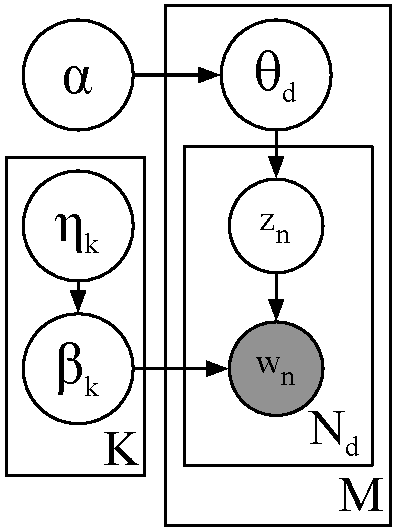
\includegraphics[width=.36\linewidth]{mrlda/lda_model}}
	\only<2>{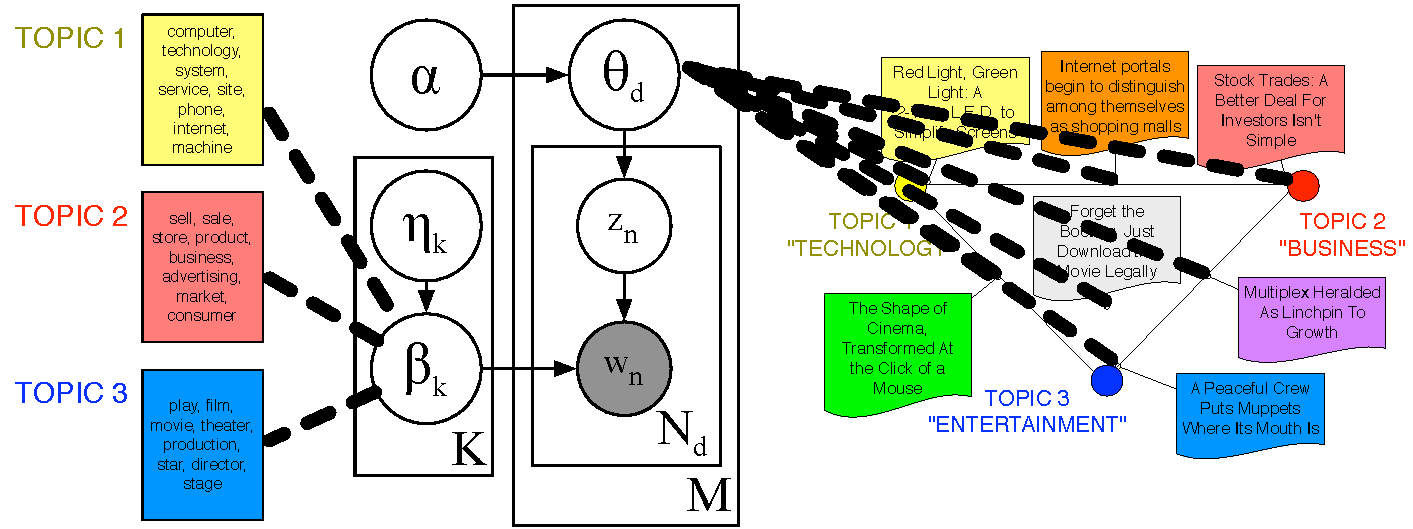
\includegraphics[width=\linewidth]{mrlda/lda_graphmod_nyt}}
	\end{center}
\end{frame}

\begin{frame}
	\frametitle{Inference}
	
	\begin{columns}
		\column{.4\linewidth}

			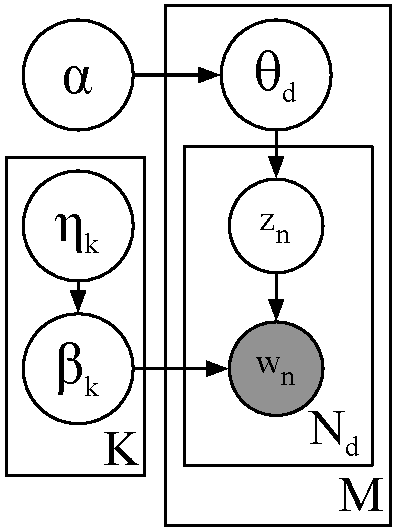
\includegraphics[width=0.9\linewidth]{mrlda/lda_model}
		\column{.6\linewidth}
			\begin{itemize}
				\item Generative models tell a story of how your data came to be
				\item There are missing pieces to that story (e.g. the topics)
				\item Statistical inference fills in the missing pieces
				\pause
				\item Hard problem - requires looking at the entire dataset
				\item Why we need large scale solutions
				\pause
				\item Use MapReduce!
			\end{itemize}
	
	\end{columns}


\end{frame}

\begin{frame}

	\frametitle{Inference}

	\begin{columns}
	
		\column{.5\linewidth}

	\begin{block}{Variational}
	\only<1>{
		\begin{itemize}
			\item Few, expensive iterations
			\item Deterministic
			\item Conjugate easier, tractable without
			\item Easy convergence diagnosis
		\end{itemize}
	}
	\end{block}
	
	\only<2->{
	
		\begin{itemize}
			\small		
			\item First LDA implementation \cite{blei-03}
			\item Master-Slave LDA \cite{nallapati-07}
			\item Apache Mahout
		\end{itemize}
	
	}
	
	\column{.5\linewidth}

	\begin{block}{MCMC / Gibbs}
	\only<1>{
		\begin{itemize}
			\item Many, cheap iterations
			\item Random
			\item Effective for {\bf conjugate} distributions
			\item Tricky convergence diagnosis
		\end{itemize}	
	}
	\end{block}
	
	\only<2->{
		\begin{itemize}
			\small
			\item Popular \cite{griffiths-04}
			\item Sparsity helps \cite{yao-09}
			\item Assume shared memory? \cite{asuncion-09}
			\item YahooLDA \cite{smola-10}
		\end{itemize}
	
	}
	
	\end{columns}
\end{frame}

\begin{frame}
	\frametitle{Expectation Maximization Algorithm}
	
	\begin{itemize}
		\item Input: $z$ (hidden variables), $\xi$ (parameters), $D$ (data)
		\item Start with initial guess of $z$, parameters $\xi$
		\item Repeat
		\begin{itemize}
			\item \only<2->{\alert<2> {\bf E-Step}} Compute the expected value of latent variables $z$ 		
			\item \only<3->{\alert<3>{\bf M-Step}} Compute the parameters $\xi$ that maximize likelihood $L$ (use calculus)
		\end{itemize}
		\item With each iteration, objective function $L$ goes up
	\end{itemize}

\end{frame}

\begin{frame}
	\frametitle{Theory}

	\begin{itemize}
		\item Sometimes you can't actually optimize $L$
		\item So we instead optimize a lower bound based on a ``variational'' distribution $q$
\begin{equation}
  \elbo = \e{q}{\log \left(p(\mbox{D} | Z) p(Z | \xi) \right) } - \e{q}{\log q(Z)}
  \label{eq:elboexpec}
\end{equation}
	\item $L - \elbo = KL(q || p)$
	\item This is called variational EM (normal EM is when $p = q$)
	\item Makes the math possible to optimize $\elbo$
	\end{itemize}

\end{frame}


\begin{frame}[fragile]

	\frametitle{Variational distribution}



\begin{figure}[htb]
\begin{center}
\subfigure[LDA]{
  \label{fig:ldamodel}
  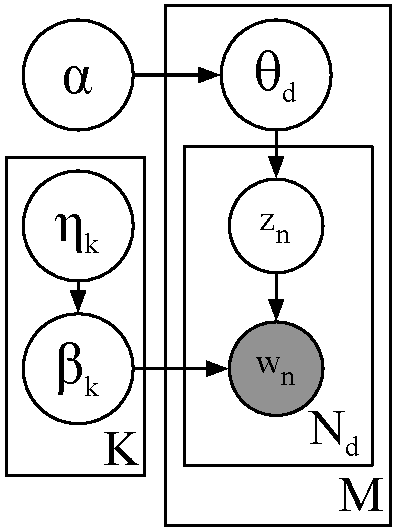
\includegraphics[width=0.40\linewidth]{mrlda/lda_model}
}
\subfigure[Variational]{
  \label{fig:variational}
	\only<1>{  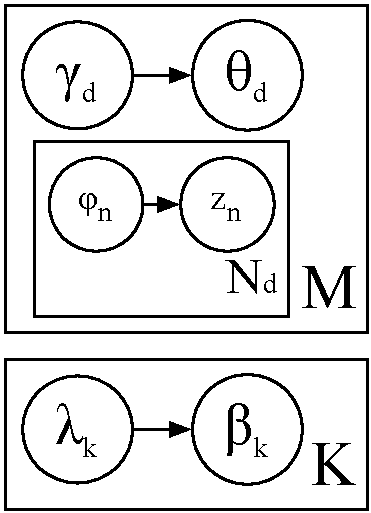
\includegraphics[width=0.35\linewidth]{mrlda/lda_variational}}
	\only<2>{ 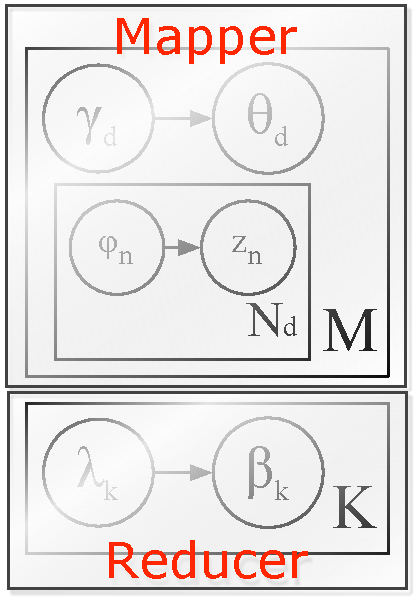
\includegraphics[width=0.35\linewidth]{mrlda/lda_variational_labeled}}
}
\end{center}
\end{figure}

\end{frame}

\begin{frame}

\frametitle{Updates - Important Part}

\begin{columns}

\column{.5\linewidth}

\begin{itemize}
	\item $\phi$ How much the $n^{th}$ word in a document expressed topic $k$ \only<2->{ \alert<2>{ (Mapper)}}
	\item $\gamma_{d,k}$ How much the $k^{th}$ topic is expressed in a document $d$ \only<2->{ \alert<2>{ (Mapper)}}
	\item $\beta_{v,k}$ How much word $v$ is associated with topic $k$ \only<3->{ \alert<3>{ (Reducer)}}
\end{itemize}

\column{.5\linewidth}

\begin{align*}
\phi_{d, n, k} & \propto \beta_{w_{d,n}, k} \cdot e^{\digam{\gamma_{k}}}\\
\gamma_{d,k} & = \alpha_{k} + \sum_{n=1}^{N_d} \phi_{d,n, k}, \\
\beta_{v, k} & \propto \eta + \sum_{d=1}^{C} ( w^{(d)}_v \phi_{d, v, k})
\end{align*}

\end{columns}

\alert<4>{
\begin{center}
	This is the algorithm!
\end{center}
}

\end{frame}

\begin{frame}
	\frametitle{Other considerations}
	
	\begin{itemize}
		\item Thus far, no difference from Mahout or \cite{nallapati-07}
		\item Computing objective function $\elbo$ to assess convergence
		\item Updating hyperparameters
		\begin{itemize}
			\item Many implementations don't do this
			\item Critical for topic quality and good likelihood
		\end{itemize}
	\end{itemize}
\end{frame}

\begin{frame}

\frametitle{Objective Function}

Expanding Equation~\ref{eq:elboexpec} gives us
$\elbo(\gamma, \phi; \alpha, \beta)$ for one document:
\begin{scriptsize}
\begin{align*}
\mathcal{L}(\gamma, \phi; \alpha, \beta) & = \sum_{d=1}^C \mathcal{L}_d(\gamma, \phi; \alpha, \beta)\\
& = \explain{Driver}{\sum_{d=1}^C \mathcal{L}_d(\alpha)} + \explain{computed in Reducer}{\sum_{d=1}^C (\explain{computed in mapper}{\mathcal{L}_d(\gamma, \phi)  + \mathcal{L}_d(\phi) + \mathcal{L}_d(\gamma)})},
\end{align*}
\end{scriptsize}
%where
%\begin{scriptsize}
%\begin{align*}
%\only<1> { \mathcal{L}_d(\alpha) & = \log \G{\sum_{k=1}^K \alpha_k} - \sum_{i=1}^K \log \G{\alpha_k}, }
%\only<2> { \mathcal{L}_d(\gamma, \phi) & = \sum_{k=1}^K \left[ \sum_{v=1}^V \phi_{v, k} -
%  \sum_{v=1}^V \phi_{v, k} w_v \right] \left[
%\digam{\gamma_k}-\digam{\sum_{i=1}^K \gamma_i} \right], }
%\only<3> {\mathcal{L}_d(\phi) & = \sum_{v=1}^V \sum_{k=1}^K \phi_{v, k} (\log \phi_{v, k} + \sum_{i=1}^V w_i \log \beta_{i, k}),}
%\only<4> { \mathcal{L}_d(\gamma) & = - \log \G{\sum_{k=1}^K \gamma_k} + \sum_{k=1}^K \log \Gamma{\gamma_k} }
%\end{align*}
%\end{scriptsize}
\end{frame}

\begin{frame}
	\frametitle{Updating hyperparameters}

We use a
Newton-Raphson method which requires the Hessian matrix and the gradient,
\begin{align*}
\alpha_{\mathsf{new}} = \alpha_{\mathsf{old}} - \mathcal{H}^{-1}(\alpha_{\mathsf{old}}) \cdot g(\alpha_{\mathsf{old}}),
\end{align*}
\pause
where the Hessian matrix $\mathcal{H}$ and gradient $g(\alpha)$ are
\begin{align*}
\mathcal{H}(k, l)  = & \delta(k, l) C \ddigam{\alpha_k} - C
\ddigam{\sum_{l=1}^K \alpha_l}, \\
g(k)  = &\explain{\footnotesize{computed in driver}}{C \left( \digam{
      \displaystyle \sum_{l=1}^K \alpha_l} -
  \digam{\alpha_k} \right) } + \explain{\footnotesize{computed in reducer}}{ \displaystyle \sum_{d=1}^C
  \explain{\footnotesize{computed in mapper}}{\digam{\gamma_{d, k}} -
    \digam{ \displaystyle \sum_{l=1}^K \gamma_{d, l}}} }.
\end{align*}

\begin{block}{Complexity}
	Removing document-dependence: update $O(K^2)$ in the driver
\end{block}

\end{frame}

\begin{frame}

\begin{center}
	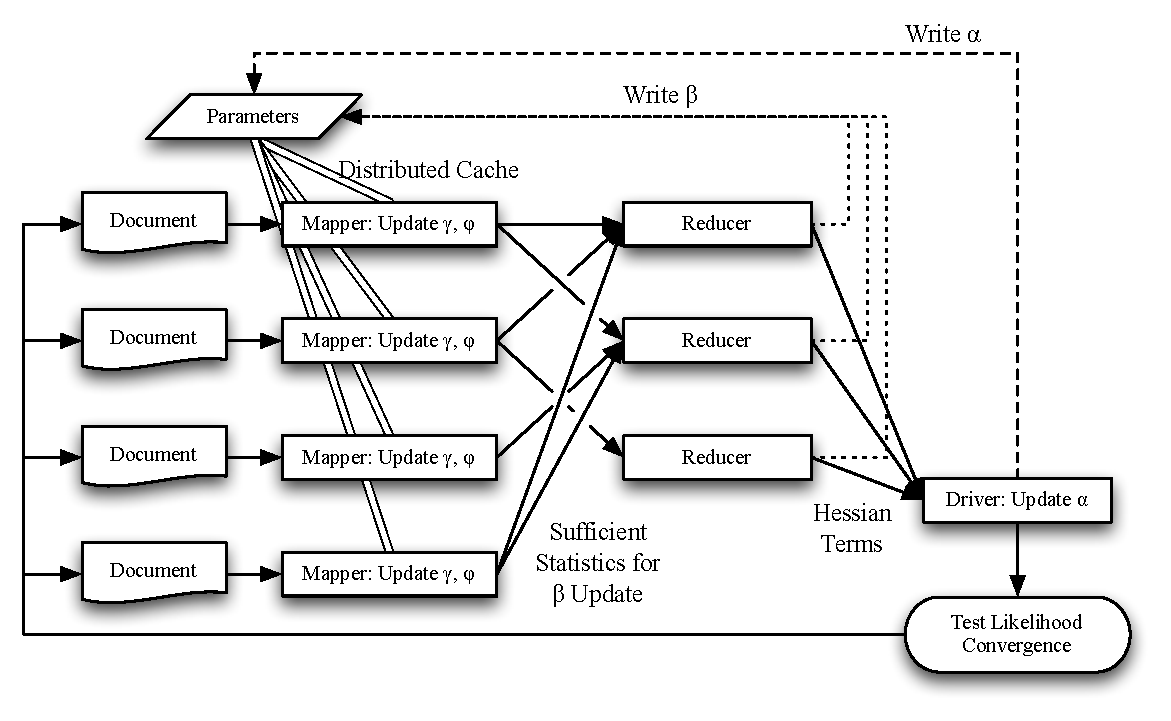
\includegraphics[width=0.8\linewidth]{mrlda/workflow}
\end{center}

\end{frame}



\begin{frame}
	\frametitle{Other implementation details}
	
	\begin{itemize}
		\item Computing $\Psi$ function is expensive, so we cache / approximate values \only<2->{\begin{itemize} \item Always helps \end{itemize}}
		\item The number of intermediate values swamp the system, so we employ in-mapper combiners~\cite{lin-10} \only<2->{\begin{itemize} \item Only helps with many topics\end{itemize}}
		\item Initialization \only<2->{\begin{itemize} \item Helps in first iterations\end{itemize}}
	\end{itemize}

\end{frame}

\begin{frame}
	\frametitle{Comparison with Mahout}
	
	\centering
	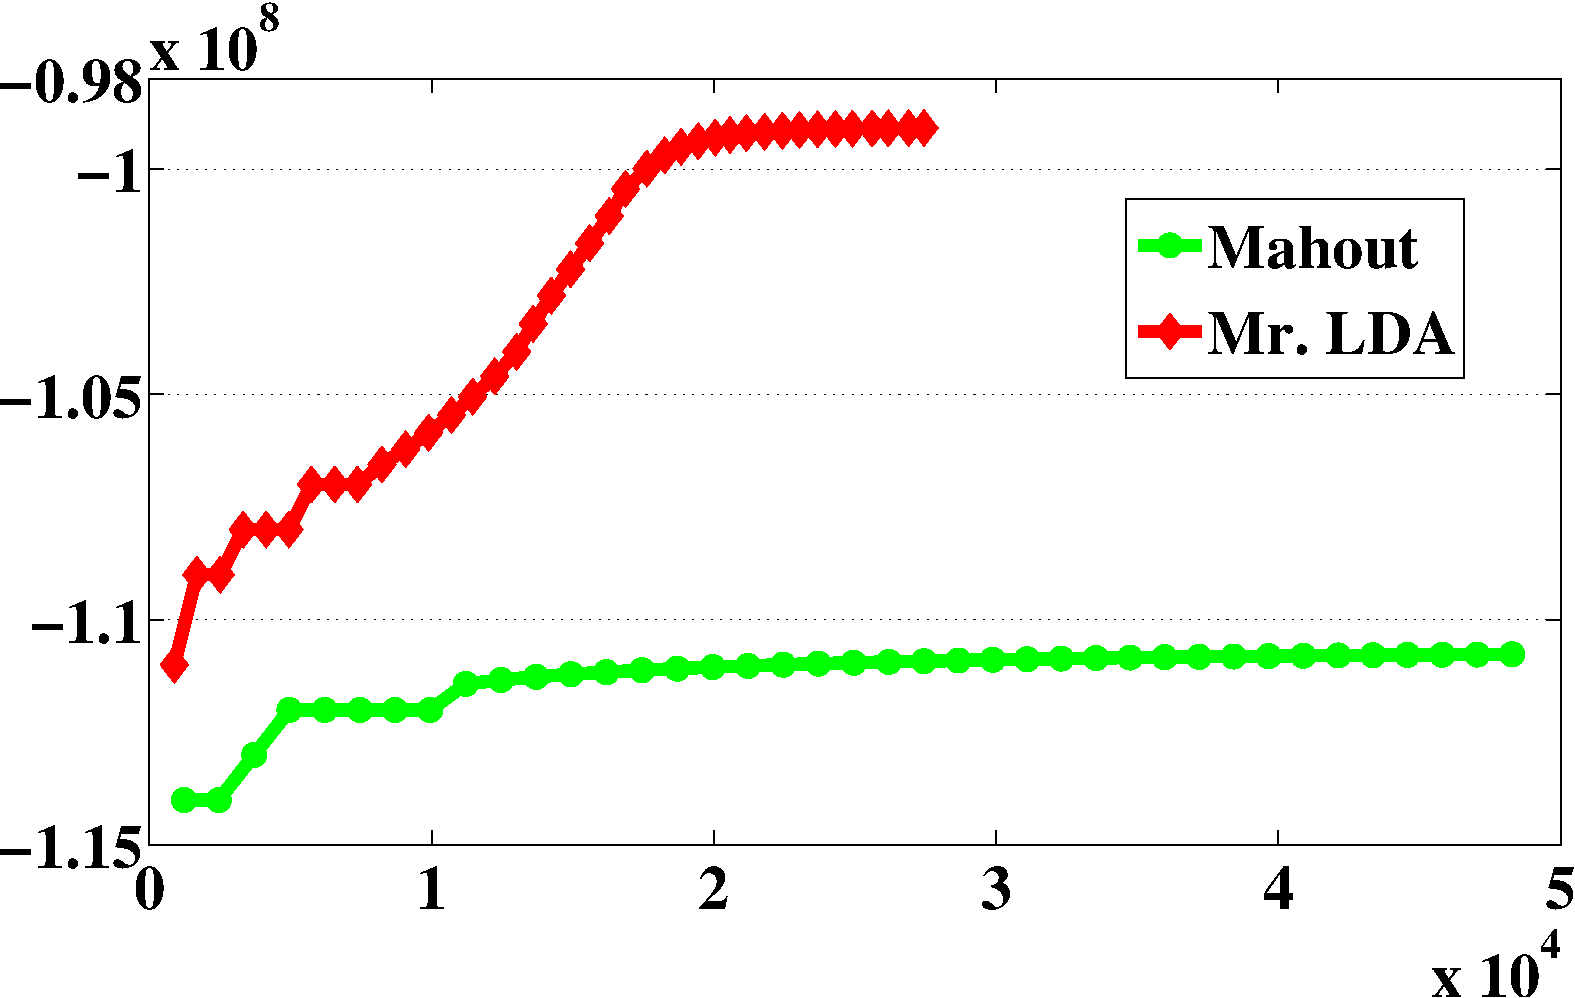
\includegraphics[width=0.95\linewidth]{mrlda/bespin-topic-100} \\
	Held-out likelihood vs. time (sec) \\
	TREC (100 topics, 500k documents)
	

\end{frame}

\section{Extensions}

\begin{frame}

	\frametitle{How are psychological factors expressed in blogs?}

	\begin{itemize}
		\item Linguistic Inquiry in Word Count~\cite{pennebaker-99}
		\item Example psychological processes:
		\begin{itemize}
			\item Anger: hate, kill, annoyed
			\item Negative Emotions: hurt, ugly, nasty
		\end{itemize}
		\item What words cooccur with these words in a particular \emph{corpus}?
		\pause
		\item Use LIWC categories as an informed prior to ``seed'' topics
		\begin{align*}
\beta_{v, k} & \propto \eta_{v,k} + \sum_{d=1}^{C} ( w^{(d)}_v \phi_{d, v, k})
\end{align*}
	\pause
	\item Not possible in SparseLDA-based models
	\end{itemize}


\end{frame}

\begin{frame}
	\frametitle{Workflow for Informed Prior}
	
	\centering
	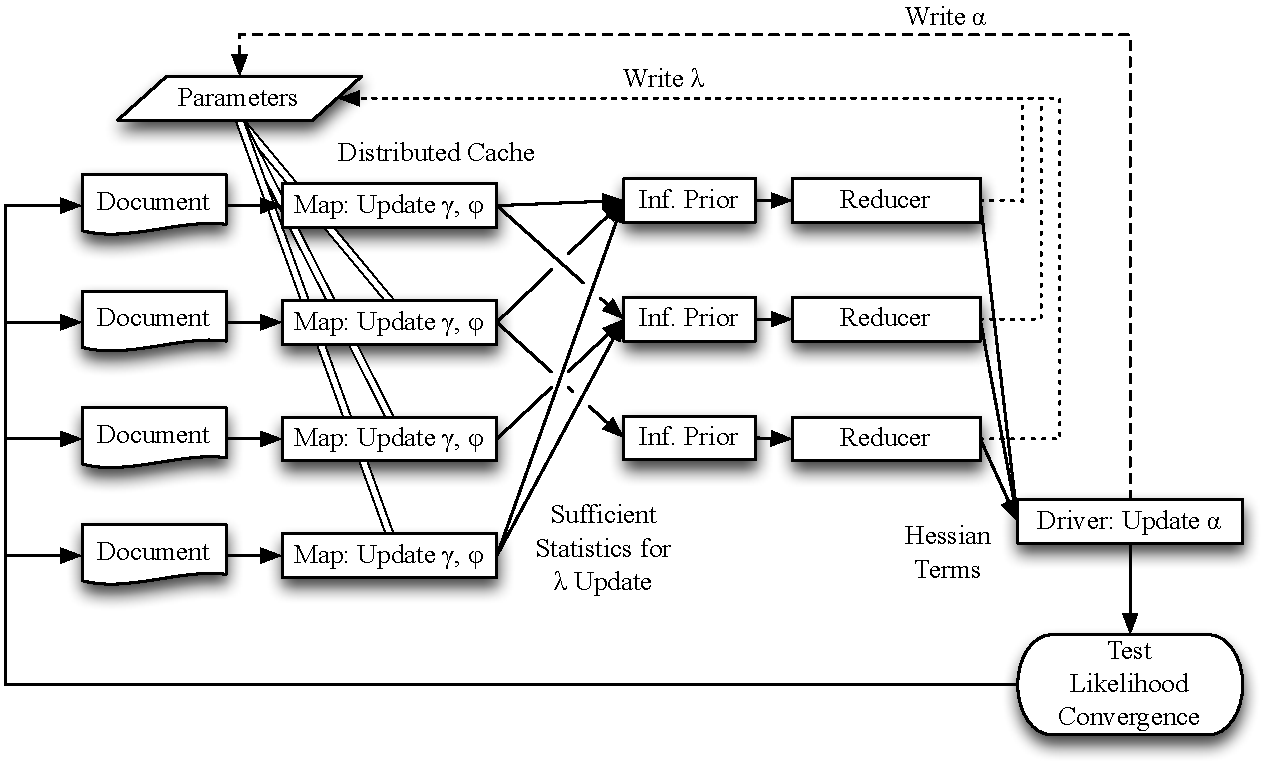
\includegraphics[width=0.8\linewidth]{mrlda/workflow_informed}
	
\end{frame}


\begin{frame}

\frametitle{Psychologically-Informed Topics from Blogs}

\centering
\scriptsize{
\begin{tabular}{p{1.3cm} p{1.3cm} p{1.3cm} p{1.0cm} p{0.8cm} p{0.7cm} p{1.0cm} p{1.0cm} p{0.8cm} p{1.0cm} p{0.8cm} p{0.9cm}}
%\footnotesize{
%\begin{tabular}{p{0.45cm} | p{1.23cm} p{1.213cm} p{1.213cm} p{1.05cm} p{0.85cm} p{0.7cm} p{1.23cm} p{1.22cm} p{0.9cm} p{1.1cm} p{1.0cm} p{1.1cm}}
\hline
Affective Processes & Negative Emotions & Positive Emotions & Anxiety & Anger & Sadness \\
\hline
 easili & sorri & lord & bird & iraq & level \\
 dare & crappi & prayer & diseas & american & grief \\
 truli & bullshit & pray & shi & countri & disord  \\
 lol & goddamn & merci & infect & militari & moder  \\
 needi & messi & etern & blood & nation & miseri \\
 jealousi & shitti & truli & snake & unit & lbs \\
 friendship & bitchi & humbl & anxieti & america & loneli  \\
 betray & angri & god & creatur & force & pain \\
\hline
\end{tabular}} \\
Using 50 topics on Blog Authorship corpus~\cite{koppel-06}

\end{frame}


\begin{frame}
	\frametitle{Polylingual LDA}
	
	\begin{columns}
		\column{.4\linewidth}
			\begin{itemize}
				\item Assumes documents have multiple ``faces''~\cite{mimno-09}
				\item Topics also assumed to have per-language distribution
				\item As long as documents talk about the same thing, learns consistent topics across languages
				\item First variational inference algorithm
			\end{itemize}
		\column{.6\linewidth}

			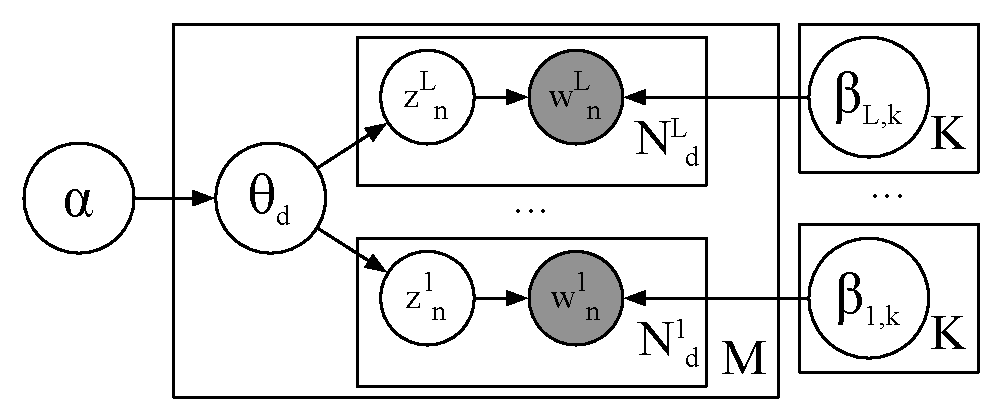
\includegraphics[width=0.9\linewidth]{mrlda/polylda}
	
	\end{columns}
	
\end{frame}


\begin{frame}
	\frametitle{Workflow for Polylingual LDA}
	
	\centering
	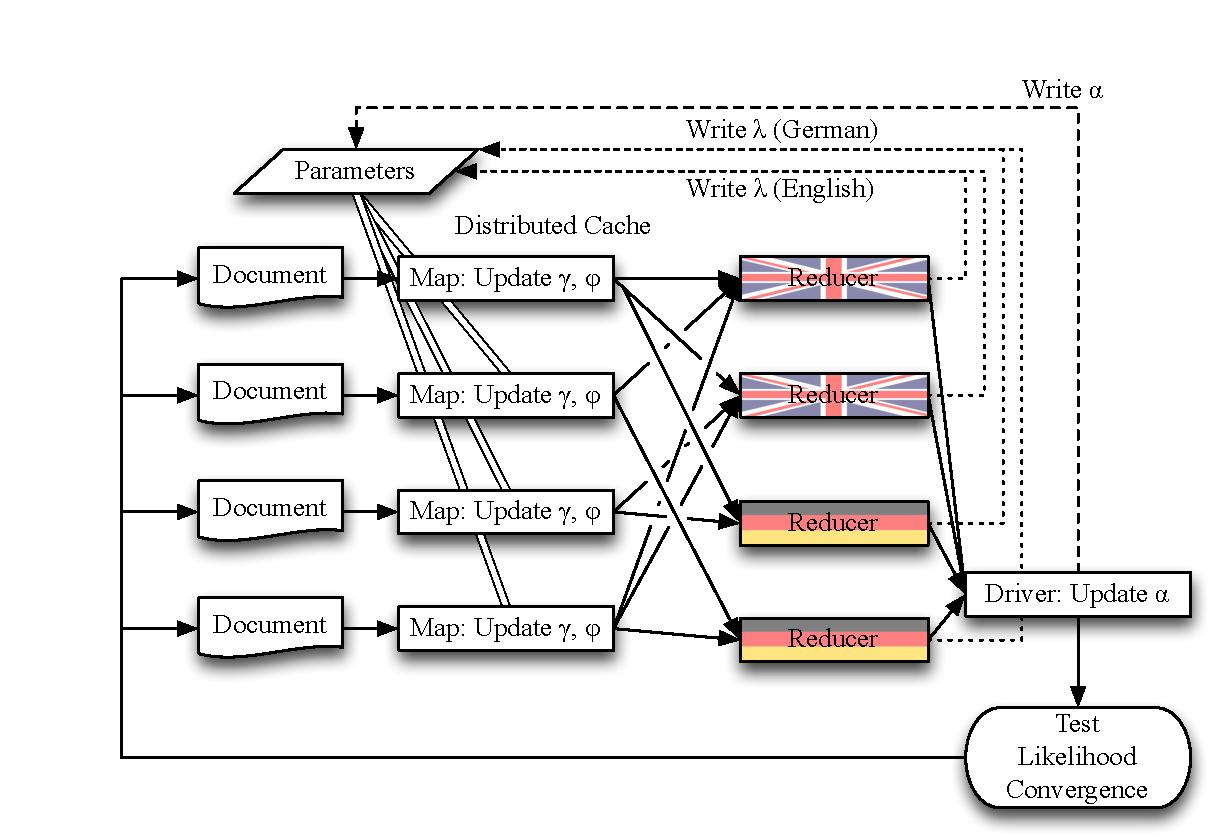
\includegraphics[width=0.8\linewidth]{mrlda/workflow_multilingual}
	
\end{frame}

\begin{frame}

\frametitle{Aligned topics from all of Wikipedia}

\center
\scriptsize{
\begin{tabular}{c | p{1cm} p{1.2cm} p{1.2cm} p{1.3cm} p{0.55cm} p{1.0cm} p{1.0cm} p{1.1cm} }
\hline
\multirow{10}{*}{\begin{sideways}English\end{sideways}}
& game & opera & greek & league & said & italian & soviet \\
& games & musical & turkish & cup & family & church & political\\
& player & composer & region & club & could & pope & military\\
& players & orchestra & hugarian & played & childern & italy & union\\
& released & piano & wine & football & death & catholic & russian \\
& comics & works & hungary & games & father & bishop & power \\
& characters & symphony & greece & career & wrote & roman & israel \\
& character & instruments & turkey & game & mother & rome & empire \\
& version & composers & ottoman & championship & never & st & republic \\
\hline
\multirow{10}{*}{\begin{sideways}German\end{sideways}}
 & spiel & musik & ungarn & saison & frau & papst & regierung \\
& spieler & komponist & turkei & gewann & the & rom & republik \\
& serie & oper & turkischen & spielte & familie & ii & sowjetunion \\
& the & komponisten & griechenland & karriere & mutter & kirche & kam \\
& erschien & werke & rumanien & fc & vater & di & krieg \\
& gibt & orchester & ungarischen & spielen & leben & bishof & land \\
& commics & wiener & griechischen & wechselte & starb & italien & bevolkerung \\
& veroffentlic & komposition & istanbul & mannschaft & tod & italienisch & ende \\
& 2 & klavier & serbien & olympischen & kinder & konig & reich \\
\hline
\end{tabular}
}

\end{frame}

\begin{frame}
	\frametitle{Which large-scale implementation is right for me?}
	
	\begin{itemize}
		\item Yahoo LDA~\cite{smola-10}
			\begin{itemize}
				\item Fastest
				\item Sparse Gibbs sampling 
				\item Great when you can use \texttt{memcached}
			\end{itemize}
		\item Mahout
			\begin{itemize}
				\item Variational
				\item Simplest
			\end{itemize}			
		\item {\bf \textsc{Mr LDA}}
		\begin{itemize}
			\item Designed for extensibility
			\item Multilingual
			\item Hyperparameter updating~\cite{wallach-09b}
			\item Likelihood monitoring
		\end{itemize}
	\end{itemize}


\end{frame}

\begin{frame}

	\frametitle{Conclusion}

	\begin{itemize}
		\item \textsc{Mr LDA}: A scalable implementation for topic modeling
		\item Extensible variational inference
		\item Next steps
		\begin{itemize}
			\item Supporting more modeling assumptions (including non-conjugacy)
			\item Nonparametrics (over topics and vocabulary)
			\item Multiple starts
		\end{itemize}

	\begin{block}{Download the Code}
		\url{http://mrlda.cc}
	\end{block}

	\end{itemize}

\end{frame}
